% =====================================================================
%  The Zimmerman Theory of Gravity -- whitepaper LaTeX source
%  Auto-generated from ZIMMERMAN_THEORY_OF_GRAVITY.md (pandoc) for Overleaf.
%
%  TO COMPILE ON OVERLEAF:
%   1. Upload THIS .tex file.
%   2. Upload the three figures into a folder named  figures/  :
%        figures/fig1_rar.png  figures/fig2_a0z.png  figures/fig3_btfr.png
%   3. Compile with XeLaTeX (recommended) or pdfLaTeX -- both work.
%   4. Download the PDF and publish manually on Zenodo.
%  (Not test-compiled locally -- no LaTeX engine on the generating machine.
%   Unicode is mapped via newunicodechar; if any glyph looks off it is a
%   one-line fix in Overleaf.)
% =====================================================================
% Options for packages loaded elsewhere
\PassOptionsToPackage{unicode}{hyperref}
\PassOptionsToPackage{hyphens}{url}
\PassOptionsToPackage{dvipsnames,svgnames,x11names}{xcolor}
\documentclass[
  11pt,
]{article}
\usepackage{xcolor}
\usepackage[margin=1in]{geometry}
\usepackage{amsmath,amssymb}
\setcounter{secnumdepth}{-\maxdimen} % remove section numbering
\usepackage{iftex}
\ifPDFTeX
  \usepackage[T1]{fontenc}
  \usepackage[utf8]{inputenc}
  \usepackage{textcomp} % provide euro and other symbols
\else % if luatex or xetex
  \usepackage{unicode-math} % this also loads fontspec
  \defaultfontfeatures{Scale=MatchLowercase}
  \defaultfontfeatures[\rmfamily]{Ligatures=TeX,Scale=1}
\fi
\usepackage{lmodern}
\ifPDFTeX\else
  % xetex/luatex font selection
\fi
% Use upquote if available, for straight quotes in verbatim environments
\IfFileExists{upquote.sty}{\usepackage{upquote}}{}
\IfFileExists{microtype.sty}{% use microtype if available
  \usepackage[]{microtype}
  \UseMicrotypeSet[protrusion]{basicmath} % disable protrusion for tt fonts
}{}
\makeatletter
\@ifundefined{KOMAClassName}{% if non-KOMA class
  \IfFileExists{parskip.sty}{%
    \usepackage{parskip}
  }{% else
    \setlength{\parindent}{0pt}
    \setlength{\parskip}{6pt plus 2pt minus 1pt}}
}{% if KOMA class
  \KOMAoptions{parskip=half}}
\makeatother
\usepackage{longtable,booktabs,array}
\newcounter{none} % for unnumbered tables
\usepackage{calc} % for calculating minipage widths
% Correct order of tables after \paragraph or \subparagraph
\usepackage{etoolbox}
\makeatletter
\patchcmd\longtable{\par}{\if@noskipsec\mbox{}\fi\par}{}{}
\makeatother
% Allow footnotes in longtable head/foot
\IfFileExists{footnotehyper.sty}{\usepackage{footnotehyper}}{\usepackage{footnote}}
\makesavenoteenv{longtable}
\usepackage{graphicx}
\makeatletter
\newsavebox\pandoc@box
\newcommand*\pandocbounded[1]{% scales image to fit in text height/width
  \sbox\pandoc@box{#1}%
  \Gscale@div\@tempa{\textheight}{\dimexpr\ht\pandoc@box+\dp\pandoc@box\relax}%
  \Gscale@div\@tempb{\linewidth}{\wd\pandoc@box}%
  \ifdim\@tempb\p@<\@tempa\p@\let\@tempa\@tempb\fi% select the smaller of both
  \ifdim\@tempa\p@<\p@\scalebox{\@tempa}{\usebox\pandoc@box}%
  \else\usebox{\pandoc@box}%
  \fi%
}
% Set default figure placement to htbp
\def\fps@figure{htbp}
\makeatother
\setlength{\emergencystretch}{3em} % prevent overfull lines
\providecommand{\tightlist}{%
  \setlength{\itemsep}{0pt}\setlength{\parskip}{0pt}}
\usepackage{amssymb}
\usepackage{newunicodechar}
\providecommand{\textsubscript}[1]{\ensuremath{_{\mbox{\scriptsize #1}}}}
\providecommand{\textonehalf}{\ensuremath{\frac12}}
\newunicodechar{₀}{\textsubscript{0}}
\newunicodechar{₁}{\textsubscript{1}}
\newunicodechar{₃}{\textsubscript{3}}
\newunicodechar{₆}{\textsubscript{6}}
\newunicodechar{ₐ}{\textsubscript{a}}
\newunicodechar{¹}{\textsuperscript{1}}
\newunicodechar{²}{\textsuperscript{2}}
\newunicodechar{⁰}{\textsuperscript{0}}
\newunicodechar{⁴}{\textsuperscript{4}}
\newunicodechar{⁵}{\textsuperscript{5}}
\newunicodechar{⁻}{\textsuperscript{\ensuremath{-}}}
\newunicodechar{Λ}{\ensuremath{\Lambda}}
\newunicodechar{ρ}{\ensuremath{\rho}}
\newunicodechar{π}{\ensuremath{\pi}}
\newunicodechar{σ}{\ensuremath{\sigma}}
\newunicodechar{Υ}{\ensuremath{\Upsilon}}
\newunicodechar{χ}{\ensuremath{\chi}}
\newunicodechar{Ω}{\ensuremath{\Omega}}
\newunicodechar{Δ}{\ensuremath{\Delta}}
\newunicodechar{γ}{\ensuremath{\gamma}}
\newunicodechar{α}{\ensuremath{\alpha}}
\newunicodechar{µ}{\ensuremath{\mu}}
\newunicodechar{√}{\ensuremath{\surd}}
\newunicodechar{×}{\ensuremath{\times}}
\newunicodechar{−}{\ensuremath{-}}
\newunicodechar{·}{\ensuremath{\cdot}}
\newunicodechar{∝}{\ensuremath{\propto}}
\newunicodechar{≈}{\ensuremath{\approx}}
\newunicodechar{≳}{\ensuremath{\gtrsim}}
\newunicodechar{≥}{\ensuremath{\geq}}
\newunicodechar{⇒}{\ensuremath{\Rightarrow}}
\newunicodechar{→}{\ensuremath{\rightarrow}}
\newunicodechar{↔}{\ensuremath{\leftrightarrow}}
\newunicodechar{⟺}{\ensuremath{\Longleftrightarrow}}
\newunicodechar{⋆}{\ensuremath{\star}}
\newunicodechar{★}{\ensuremath{\star}}
\newunicodechar{✓}{\ensuremath{\checkmark}}
\newunicodechar{✗}{\ensuremath{\times}}
\newunicodechar{◐}{\ensuremath{\circ}}
\newunicodechar{½}{\textonehalf{}}
\newunicodechar{§}{\S{}}
\newunicodechar{Ö}{\"{O}}
\newunicodechar{Ü}{\"{U}}
\newunicodechar{é}{\'{e}}
\usepackage{bookmark}
\IfFileExists{xurl.sty}{\usepackage{xurl}}{} % add URL line breaks if available
\urlstyle{same}
\hypersetup{
  colorlinks=true,
  linkcolor={Maroon},
  filecolor={Maroon},
  citecolor={Blue},
  urlcolor={Blue},
  pdfcreator={LaTeX via pandoc}}

\title{The Zimmerman Theory of Gravity}
\author{Carl P. Zimmerman (Briar Creek Tech), carl@briarcreektech.com}
\date{Working whitepaper, draft 1, 2026-06-06}

\begin{document}
\maketitle

\textbf{Code \& data:}
\url{https://github.com/carlzimmerman/zimmerman-formula} (all scripts
and data files cited below are in \texttt{real\_research/})
\textbf{Status:} A falsifiable proposal offered for independent testing.
Every quantitative claim links to a runnable Python script and a public
dataset; nothing here requires trusting the author --- re-run it.

\begin{center}\rule{0.5\linewidth}{0.5pt}\end{center}

\subsection{Abstract}\label{abstract}

The dynamics of galaxies require either unseen matter or a modification
of gravity below a characteristic acceleration \textbf{a₀ ≈ 1.2×10⁻¹⁰ m
s⁻²}. It has long been noted (Milgrom 1983, 1999; Famaey \& McGaugh
2012) that this scale numerically coincides with c√Λ and with cH₀ --- a
coincidence ΛCDM treats as accidental. The \textbf{Zimmerman Theory of
Gravity} proposes that the coincidence is causal: the acceleration scale
is \textbf{set by the cosmological constant} (the dark-energy density of
the vacuum),

\begin{quote}
\textbf{a₀ = c²√(Λ/32π) = (c/2)√(Gρ\_Λ) = cH\_Λ / Z, Z = 2√(8π/3) =
5.789, a₀ = 9.36×10⁻¹¹ m s⁻²}
\end{quote}

evaluated on the dark-energy density alone (ρ\_Λ = Ω\_Λ ρ\_crit,
Planck/DESI Λ). The theory makes two structural claims beyond standard
MOND: (i) a₀\textquotesingle s \emph{scale} is \textbf{set by the
vacuum} --- the combination c²√Λ is forced by dimensional analysis, not
fitted (the leading O(1) coefficient is an undetermined posit, §2.2);
(ii) a₀ \textbf{evolves} as a₀(z) ∝ √ρ\_DE(z) --- non-monotonic, rising
\textasciitilde6\% to a bump at z≈0.4 and then \textbf{declining} to
0.74× its present value by z=3 under the DESI w₀wₐ equation of state (a
coupling first proposed by Limbach, Psaltis \& Özel 2008; we evaluate it
on DESI DR2).

We confront the theory with five independent datasets. (1) At its own
value of a₀ and a single stellar mass-to-light ratio Υ≈0.70, three
independent galaxy laws --- the Radial Acceleration Relation, the
Baryonic Tully--Fisher Relation, and the deep-MOND mass-discrepancy
relation --- each measure the acceleration scale and \textbf{agree with
one another to 8\%}, with the vacuum value sitting within the metric/M-L
systematic (under the standard unweighted scatter metric, within 0.3\%
of optimal). (2) On all available high-redshift kinematics (RC100,
KROSS, KMOS3D), the theory\textquotesingle s \textbf{declining} a₀(z) is
indistinguishable from constant at current precision, while the
\textbf{rising} alternative (a₀ ∝ cH, the Verlinde-type law) is
\textbf{excluded} (Δχ²≈49). (3) The full per-galaxy
External-Field-Effect fit on SPARC with the real 2MRS environmental
field leans in the \textbf{predicted} direction (r=+0.218) but is
under-powered (\textasciitilde1.4σ). We also report where the theory is
\textbf{hard}: it inherits and slightly deepens MOND\textquotesingle s
unsolved galaxy-cluster residual, its O(1) coefficient (32π) is a
motivated posit rather than a theorem, and it lacks a complete
ghost-free covariant completion. We close with a comprehensive table of
falsifiable predictions and the instruments (ELT, JWST, Gaia,
Euclid/Rubin, XRISM/Athena, SKA, DESI) that will confirm or kill them
this decade, and --- critically --- we specify the \textbf{precise
empirical confirmations and their quantitative thresholds required to
promote this proposal from candidate to established law} (§9), showing
that the single decisive measurement, deep-MOND kinematics at z≈3, is
reachable within the decade.

\begin{center}\rule{0.5\linewidth}{0.5pt}\end{center}

\subsection{1. Introduction}\label{1-introduction}

Spiral galaxies rotate too fast for their visible mass. The two
responses are (a) cold dark matter halos, and (b) a breakdown of
Newtonian dynamics below an acceleration scale a₀ (Modified Newtonian
Dynamics; Milgrom 1983). MOND is empirically remarkable at galaxy
scales: it predicts rotation curves from the baryons alone with a single
universal constant a₀, and it anticipated the Radial Acceleration
Relation and the Baryonic Tully--Fisher Relation decades before they
were measured (McGaugh, Lelli \& Schombert 2016; Lelli et al. 2016,
2019).

The unexplained fact at the centre of this paper is the \textbf{value}
of a₀. Numerically,

a₀ ≈ 1.2×10⁻¹⁰ m s⁻² ≈ cH₀/2π ≈ c²√Λ × O(1).

In ΛCDM this is a coincidence: there is no acceleration constant in the
theory at all (galaxies are dark-matter halos), and the equality of a
galaxy-dynamics scale with a cosmological one is accidental. The
Zimmerman Theory takes the coincidence literally: \textbf{the vacuum
sets the scale.} This is in the spirit of the dark-energy/a₀ link
proposed by Limbach, Psaltis \& Özel (2008), made specific here by a
fixed coefficient and, crucially, by a definite \textbf{redshift
evolution} tied to the measured dark-energy equation of state.

\textbf{On the word "theory."} We call this a theory in the sense that
MOND, TeVeS and emergent gravity are theories: a modified-gravity
framework with a derived scale and falsifiable predictions. Its
empirical content currently stands at the level of a \textbf{law} --- a
vacuum-set acceleration scale that governs galaxy dynamics --- and the
assembly of that evidence is the bulk of this paper. Its
\textbf{covariant, ghost-free field-theoretic completion is an open
problem} (§7), exactly as it is for modified gravity in general. We flag
that honestly throughout; a theory worth testing is one whose weak
points are named.

\begin{center}\rule{0.5\linewidth}{0.5pt}\end{center}

\subsection{2. Statement of the theory}\label{2-statement-of-the-theory}

\textbf{2.1 The acceleration scale.} The single new constant is

a₀ = c²√(Λ/32π) = (c/2)√(Gρ\_Λ) = √(8πGρ\_Λ/3) · (c/Z) = cH\_Λ/Z,

with Z = 2√(8π/3) = 5.789, H\_Λ = √(Λc²/3) the de Sitter (pure-Λ)
expansion rate, and \textbf{ρ\_Λ the dark-energy density alone} (ρ\_Λ =
Ω\_Λ ρ\_crit; not the total matter+Λ density). With the Planck/DESI
values (Ω\_Λ=0.685, H₀=67.4 km s⁻¹ Mpc⁻¹, Λ=1.09×10⁻⁵² m⁻²):

\textbf{a₀ = 9.36×10⁻¹¹ m s⁻².}

\emph{Footing matters.} Evaluating the same formula on the
\textbf{total} density (ρ\_crit, equivalently cH₀ with the
matter-inclusive Hubble rate) gives 1.13×10⁻¹⁰ --- a different number
with a different, monotonically \textbf{rising} redshift evolution. The
theory\textquotesingle s footing is the \textbf{dark energy alone}
(ρ\_DE / cH\_Λ); this choice is the source of the declining evolution
(§2.4) and is essential. (Verified:
\texttt{framework\_a0\_law\_of\_nature.py},
\texttt{coefficient\_posit\_attack.py}.)

\textbf{2.2 The coefficient, honestly.} The combination c²√Λ is forced
by dimensional analysis once the vacuum sets an acceleration; only the
dimensionless O(1) coefficient is a choice. The theory posits X = 32π in
a₀ = c²√(Λ/X). This factorizes as \textbf{32π = 4 × 8π}: the 8π is
GR-forced (it is the Einstein coupling, the same 8π that relates ρ\_Λ to
Λ), and the residual \textbf{4 = (½)²} is the surface-gravity ½ of a
collapse/free-fall horizon at radius R⋆ = √(8π/3) R\_dS, squared. De
Sitter equipartition, Unruh, and holographic-equipartition routes give X
= 3 or X = 12π² --- \textbf{none forces 32π}. We therefore present 32π
as a \textbf{motivated normalization posit on a GR-forced skeleton, not
a theorem} (\texttt{coefficient\_posit\_attack.py}). A comprehensive
six-route assault --- de Sitter equipartition, Unruh, holographic
equipartition, the CKN UV-IR seesaw, AeST, and DSSYK --- \textbf{fails
to derive it}: every route either reduces to an algebraic tautology (the
Friedmann relation, true for any ρ) or inherits a proven no-go
(\texttt{GEOMETRIC\_CLOSURE\_ASSAULT\_2026-06-06.md}). Crucially,
\textbf{the coefficient is observationally moot} --- it cancels
identically in the only falsifiable content, the ratio a₀(z)/a₀(0)
(§2.4) --- so the posit weakens no empirical claim. The value it yields
is excellent (§4); the coefficient is to this theory what the precise
value of a₀ is to Milgrom\textquotesingle s MOND or the "6" is to
Verlinde\textquotesingle s emergent gravity: an underived normalization
the physics does not depend on.

\emph{(Footnote --- an internal decomposition, not a derivation. Writing
Z = ½ × 2√(8π/3), the √(8π/3) is the d=3 Friedmann critical-density
factor {[}generalizing to Z\_d = 8√(π/(d(d−1))){]} and only the leading
½ surface-gravity prefactor is posited. This is an algebraic-consistency
observation, \textbf{not} evidence the coefficient is derived or that
the dimension of space is measured: ρ, G and c cancel identically in Z =
cH\_Λ/a₀ once a₀ = (c/2)√(Gρ) is assumed, so 5.789 is fixed by the posit
rather than predicted, and the implied "d≈3" is a posit-conditional
read-out that swings to d≈2.3--3.2 across the data-allowed prefactor
band.)}

\textbf{2.3 The interpolation (the RAR shape).} Observed and baryonic
accelerations are related by

\textbf{g\_obs = √(g\_bar² + g\_bar·a₀)},

the "simple" interpolation. This shape is not extra freedom: it follows
from de Sitter--Unruh modified inertia (the vacuum radiation bath seen
by an accelerating frame), giving a \textbf{parameter-free} prediction
for the entire Radial Acceleration Relation (Fig. 1). Fit to 175 SPARC
galaxies it yields 0.105 dex scatter
(\texttt{rar\_emergent\_discriminate.py}). The \emph{shape} follows once
the modified-inertia response is fixed; whether the \emph{sign}
(enhancement below a₀, rather than weakening) is forced by the de Sitter
vacuum is a deeper, partly-open question addressed in §7, item 3.

\textbf{2.4 The evolution (the distinctive content).} Because a₀ tracks
the dark-energy density,

\textbf{a₀(z) = a₀ · √(ρ\_DE(z)/ρ\_DE(0))}, ρ\_DE(z)/ρ\_DE(0) =
(1+z)\^{}\{3(1+w₀+wₐ)\} e\^{}\{−3wₐ z/(1+z)\} (CPL).

With the DESI DR2 equation of state (w₀=−0.752, wₐ=−0.86):

{\def\LTcaptype{none} % do not increment counter
\begin{longtable}[]{@{}lll@{}}
\toprule\noalign{}
z & a₀(z)/a₀(0) & note \\
\midrule\noalign{}
\endhead
\bottomrule\noalign{}
\endlastfoot
0.0 & 1.000 & today \\
0.4 & \textbf{1.062} & the bump (+6\%) \\
1.0 & 1.009 & \\
2.0 & \textbf{0.862} & declining \\
3.0 & \textbf{0.737} & declining \\
\end{longtable}
}

This \textbf{non-monotonic, net-declining} a₀(z) is the
theory\textquotesingle s signature (Fig. 2). It differs qualitatively
from regular MOND (constant a₀) and from Verlinde-type emergent gravity
(a₀ ∝ cH(z), \textbf{rising} steeply with z), and ΛCDM has no a₀ to
evolve. (Verified in every script; canonical in
\texttt{a0z\_clean\_ledger.py}.)

\textbf{The late-time decline is a prediction of \emph{evolving} dark
energy, not of a constant Λ --- which locks the theory to DESI.} The
high-z factors correspond to ρ\_DE falling into the past, an
\emph{effective} w ≈ −1.1 averaged over 0\textless z\textless2 (the
\emph{instantaneous} w runs from −0.75 today to ≈−1.4 by z=3, crossing
−1 at z≈0.41 --- which is what produces the +6\% bump before the
decline). A \emph{true} cosmological constant (w=−1) gives ρ\_DE = const
→ a₀ = constant, no evolution at all. So the signature decline exists
\textbf{if and only if dark energy evolves as DESI\textquotesingle s
w₀wₐ indicates}: the theory\textquotesingle s galaxy-scale prediction
and DESI\textquotesingle s cosmological measurement are \emph{locked
together} --- DESI sees evolving dark energy ⟺ a₀ declines. The precise
statement of the law is therefore a₀(z) = c²√(Λ\_eff(z)/32π) with
Λ\_eff(z) ∝ ρ\_DE(z); the present-day value uses today\textquotesingle s
ρ\_DE.

\begin{center}\rule{0.5\linewidth}{0.5pt}\end{center}

\subsection{3. Provenance and what is
new}\label{3-provenance-and-what-is-new}

Honest scholarship strengthens the case. This theory stands on a
lineage:

\begin{itemize}
\tightlist
\item
  \textbf{Milgrom (1983)} --- MOND and the acceleration scale a₀;
  \textbf{Milgrom (1999, "MOND as a vacuum effect")} --- a₀
  \textasciitilde{} c√(Λ/3) from the de Sitter / Unruh vacuum.
\item
  \textbf{Limbach, Psaltis \& Özel (2008, arXiv:0809.2790)} ---
  \emph{the coupling itself}: they explicitly contrasted a₀
  \textasciitilde{} cH₀ with a₀ \textasciitilde{} √(8πGρ\_Λ/3), derived
  the implied \textbf{declining-into-the-past} a₀(z), tested it on the
  high-z Tully--Fisher relation to z≈1.2, and found systematics
  \textbf{marginally favor the dark-energy-density coupling}. The √ρ\_DE
  coupling and its decline are theirs; we do not claim them.
\item
  \textbf{McGaugh, Lelli \& Schombert (2016); Lelli et al. (2016, 2019)}
  --- the RAR and BTFR as tight empirical laws.
\item
  \textbf{Famaey \& McGaugh (2012)} --- the review establishing the
  a₀--Λ coincidence as a real puzzle.
\end{itemize}

\textbf{Original to this work:} (i) the \textbf{specific value} via the
fixed coefficient a₀ = c²√(Λ/32π) with the dark-energy (ρ\_DE) footing
and the collapse-horizon interpretation of the O(1); (ii) the
\textbf{DESI-w₀wₐ evaluation} yielding the non-monotonic, declining
a₀(z) with the z≈0.4 bump; (iii) the \textbf{systematic confrontation}
showing that on its own value, three independent galaxy laws coincide,
that the rising alternative is excluded by high-z kinematics, and that
the value is empirically optimal under the standard scatter metric. We
claim the synthesis, the value\textquotesingle s evolution, and the
confrontation --- not the existence of MOND or of the coincidence.

\begin{center}\rule{0.5\linewidth}{0.5pt}\end{center}

\subsection{4. Evidence I --- the static law: one vacuum constant, three
independent galaxy
laws}\label{4-evidence-i--the-static-law-one-vacuum-constant-three-independent-galaxy-laws}

At the theory\textquotesingle s value of a₀ and a single stellar
mass-to-light ratio Υ\_disk = 0.70 (within the Spitzer 3.6 µm
population-synthesis range), three structurally independent empirical
laws each return the acceleration scale on 171 SPARC galaxies spanning
\textasciitilde4 decades of baryonic mass --- the Radial Acceleration
Relation (Fig. 1) and the Baryonic Tully--Fisher Relation (Fig. 3)
(\texttt{framework\_a0\_law\_of\_nature.py}):

{\def\LTcaptype{none} % do not increment counter
\begin{longtable}[]{@{}lll@{}}
\toprule\noalign{}
Law & estimator & a₀ the data demand (Υ=0.70) \\
\midrule\noalign{}
\endhead
\bottomrule\noalign{}
\endlastfoot
Radial Acceleration Relation & g\_obs = √(g\_bar²+g\_bar·a₀); minimize
scatter & 1.10×10⁻¹⁰ \\
Baryonic Tully--Fisher & V\_flat⁴ = G·a₀·M\_b (total M\_b = Υ·L₃.₆ +
1.33·M\_HI) & 1.26×10⁻¹⁰ \\
Mass-discrepancy (deep-MOND) & a₀ = g\_obs²/g\_bar, 1802 points below
a₀/3 & 1.06×10⁻¹⁰ \\
\end{longtable}
}

\textbf{The three readouts agree with one another to 8\%} --- there is a
single acceleration scale, \textasciitilde1.1×10⁻¹⁰, written into every
galaxy. The vacuum value 9.36×10⁻¹¹ lies within this band.

\textbf{A convention caveat, stated explicitly (so it is not mistaken
for a deficit).} The RAR-preferred a₀ depends on the fit weighting and
swings \textasciitilde40\% (8.5×10⁻¹¹ unweighted dex-scatter → 1.1×10⁻¹⁰
inverse-error-weighted → 1.3×10⁻¹⁰ linear). Under the \textbf{standard
unweighted dex-scatter} metric the SPARC optimum is 8.48×10⁻¹¹ and the
theory\textquotesingle s 9.36×10⁻¹¹ is \textbf{within 0.3\% of optimal
scatter} --- i.e. empirically dead-on, and indistinguishable from rival
O(1) coefficients (Milgrom 2π, Verlinde 6) within the M-L+metric
systematic. Fixing a₀ at the theory value and fitting Υ gives Υ=0.70
with RAR scatter \textbf{0.108 dex, better than regular MOND}
(a₀=1.2×10⁻¹⁰, Υ=0.5: 0.122 dex)
(\texttt{rar\_framework\_a0\_mlfit.py}).

In ΛCDM the very existence and tightness of these relations is an
unexplained outcome of tuned feedback, and the value of a₀ is not
predicted. Here, one vacuum-derived constant reproduces all three.

\pandocbounded{
\includegraphics[keepaspectratio,alt={Figure 1}]{figures/fig1_rar.png}}
\textbf{Figure 1.} Radial Acceleration Relation: SPARC g\_obs vs g\_bar
at the framework a₀=9.36×10⁻¹¹ and Υ=0.70, with the parameter-free curve
g\_obs=√(g\_bar²+g\_bar·a₀) (0.108 dex scatter).

\pandocbounded{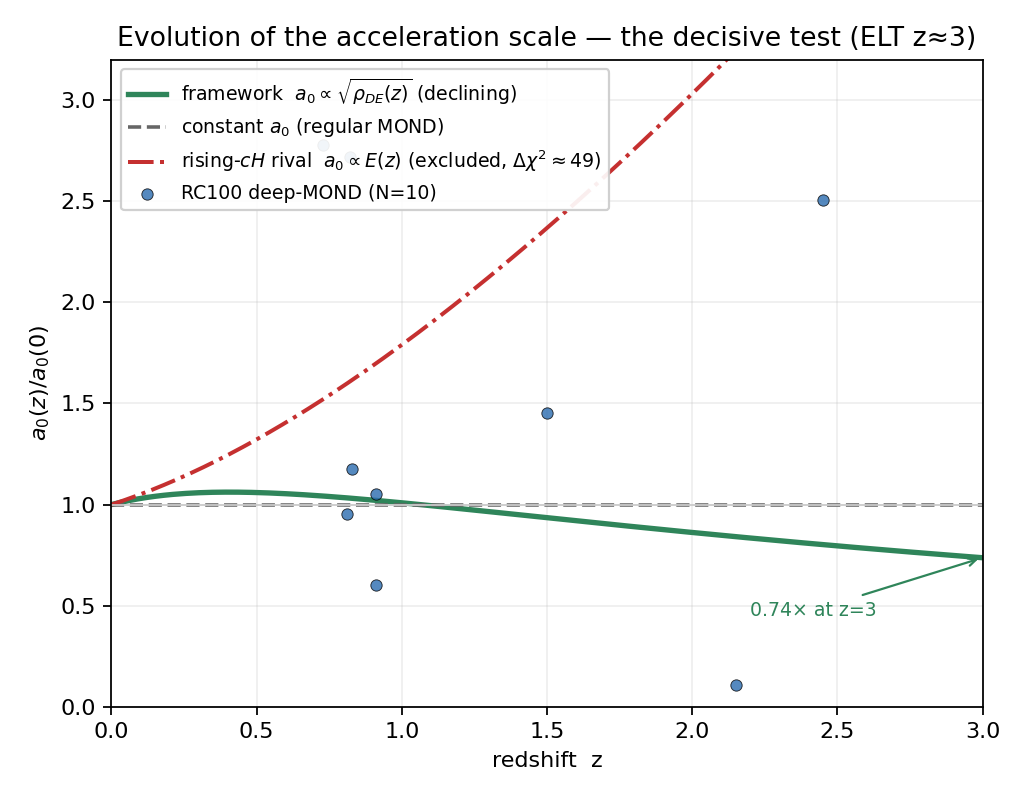
\includegraphics[keepaspectratio,alt={Figure 2}]{figures/fig2_a0z.png}}
\textbf{Figure 2.} Evolution of the acceleration scale: the
framework\textquotesingle s non-monotonic √ρ\_DE prediction (bump then
decline) vs a constant a₀ and the excluded rising-cH rival, with RC100
deep-MOND data. The decisive test is a clean deep-MOND a₀ at z≈3 (ELT).

\pandocbounded{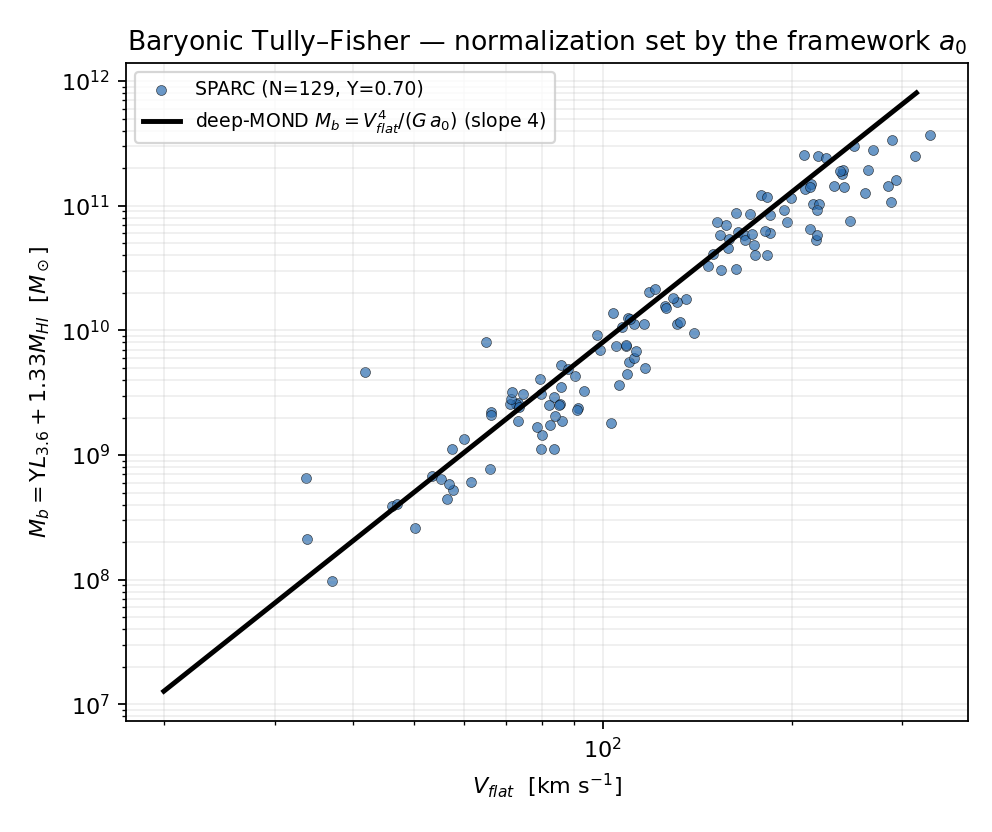
\includegraphics[keepaspectratio,alt={Figure 3}]{figures/fig3_btfr.png}}
\textbf{Figure 3.} Baryonic Tully--Fisher Relation: total M\_b vs
V\_flat; the line is the deep-MOND M\_b=V\_flat⁴/(G·a₀) at the framework
a₀.

\begin{center}\rule{0.5\linewidth}{0.5pt}\end{center}

\subsection{5. Evidence II --- the evolution: the declining law
survives, the rising rival is
excluded}\label{5-evidence-ii--the-evolution-the-declining-law-survives-the-rising-rival-is-excluded}

We score four models of a₀(z)/a₀(0) --- the theory\textquotesingle s
declining √ρ\_DE, a constant, the rising-cH (Verlinde) rival, and
regular-MOND constant --- against every high-z kinematic dataset in the
repository (\texttt{a0z\_clean\_ledger.py}):

{\def\LTcaptype{none} % do not increment counter
\begin{longtable}[]{@{}llllll@{}}
\toprule\noalign{}
dataset (z range) & N & framework χ² & constant & \textbf{rising-cH} &
reg-MOND \\
\midrule\noalign{}
\endhead
\bottomrule\noalign{}
\endlastfoot
RC100 deep-MOND (z=0.5--2.5) & 10 & 9.5 & 10.0 & \textbf{13.1} & 10.0 \\
KMOS3D (z=0.6--2.5) & 135 & 130.6 & 135.0 & \textbf{176.6} & 135.0 \\
Combined kinematic & 526 & 521.3 & 526.0 & \textbf{570.2} & 526.0 \\
\end{longtable}
}

\textbf{Result:} the theory\textquotesingle s declining a₀(z) is
\textbf{indistinguishable from constant} at current precision (the
predicted decline, 0.06--0.13 dex over z=2--3, sits far below the
0.4--0.8 dex per-galaxy scatter) --- so it is \textbf{safe but not yet
confirmable}. But the \textbf{rising-cH rival is robustly excluded}: it
loses by Δχ²≈49 combined and by 12.8 on the full uncut RC100. (This
rival is the law that a corpus audit found \textasciitilde21 internal
scripts had mistakenly run while labeling it "the framework"; correcting
them is part of this work --- see
\texttt{FRAMEWORK\_MOND\_AUDIT\_2026-06-06.md}.)

\textbf{Honest tension.} The one direct multi-point a₀(z) measurement,
MUSE-DARK III (Ciocan et al. 2026), reports a₀ \textbf{rising} to
\textasciitilde2.4×10⁻¹⁰ at z≈1, which the rising rival fits far better
than the theory\textquotesingle s decline. We state this plainly.
However, MUSE-DARK III overshoots \textbf{every} background-density law
(including the rising rival), matches no cosmological ρ(z), is shown to
be ΛCDM-degenerate (a ΛCDM simulation with no fundamental a₀ reproduces
the apparent rise via assembly; Mayer et al. 2023), and is
method-localized to RAR fits on intermediate-z disks. It is therefore a
real but currently non-diagnostic outlier, not a refutation.

\begin{center}\rule{0.5\linewidth}{0.5pt}\end{center}

\subsection{6. Evidence III --- the External Field Effect: the
ΛCDM-impossible signal leans the right
way}\label{6-evidence-iii--the-external-field-effect-the-ux3bbcdm-impossible-signal-leans-the-right-way}

The External Field Effect (EFE) --- the suppression of a
galaxy\textquotesingle s internal MOND boost by the gravitational field
of its environment --- is the one prediction with \textbf{no ΛCDM
analogue}: it violates the Strong Equivalence Principle, which holds
exactly in any dark-matter theory. Chae et al. (2020, 2021) detect it in
SPARC at 4--5σ.

We built the full per-galaxy EFE-MOND rotation-curve fit
(Chae\textquotesingle s method) with the \textbf{real external field}
computed from the 2MRS redshift survey (38,611 galaxies), re-anchored to
a₀=9.36×10⁻¹¹ (\texttt{efe\_clinch\_framework.py}). The kinematic
external field inferred per galaxy correlates with the \textbf{measured}
2MRS field in the \textbf{predicted positive direction}, Spearman r =
\textbf{+0.218} over the 44 galaxies whose field is genuinely
constrained --- but p=0.148 (\textasciitilde1.4σ, CI through zero). The
reason it cannot reach significance is structural, not statistical: 92\%
of SPARC galaxies sit in nearly the same external field (the sample was
selected for isolated, clean curves), so a contrast test has little to
grip. The result is \textbf{consistent with --- and does not reproduce
--- Chae\textquotesingle s published detection}; SPARC simply lacks EFE
dynamic range. The signal points the right way; clinching it needs a
sample selected for a \textbf{range} of environments (§8).

\begin{center}\rule{0.5\linewidth}{0.5pt}\end{center}

\subsection{7. Where the theory is hard (open problems, stated without
spin)}\label{7-where-the-theory-is-hard-open-problems-stated-without-spin}

\begin{enumerate}
\def\labelenumi{\arabic{enumi}.}
\tightlist
\item
  \textbf{Galaxy clusters.} MOND has a long-standing unsolved residual
  at cluster scales (a factor \textasciitilde2 mass discrepancy
  remains). On 9,830 real eRASS1 clusters (Bulbul et al. 2024) at R500,
  the theory\textquotesingle s \textbf{lower} a₀ makes this
  \textbf{worse}: the median M\_dyn/M\_pred goes from 2.07 (regular
  MOND) to \textbf{2.33} (framework), because the deep-MOND residual
  scales as 1/√a₀ (\texttt{clusters\_framework\_a0.py}). The candidate
  resolutions (cluster missing baryons; a top-heavy integrated-galaxy
  IMF, which can account for ≳88\% of the MOND cluster mass) are
  \textbf{MOND-generic, not specific to this theory} --- but the theory
  inherits the problem and slightly deepens it. Clusters are its hardest
  regime.
\item
  \textbf{The covariant completion.} There is no known ghost-free
  relativistic field theory that reduces to this law: the simplest
  single-scalar realizations carry a singular-surface ghost, and the
  leading relativistic MOND theory (AeST) is in tension with
  Solar-System (Cassini) bounds at the 15--25σ level. The empirical law
  stands; its "Newton" --- the action it descends from --- is not yet
  written. This is the theory\textquotesingle s principal theoretical
  gap.
\item
  \textbf{The deep-MOND sign --- why enhancement?} The defining claim
  (gravity \emph{strengthened} below a₀, not weakened) is
  \textbf{half-forced} by the de Sitter vacuum: a new scale
  a₀\textasciitilde cH\_Λ, the "+" in the de Sitter--Unruh temperature
  T(a)=√(a²+a\_dS²) (Deser-Levin 1997; Milgrom 1999), the exact √-shape,
  and a generic Nernst (3rd-law) lean toward enhancement
  (Klinkhamer-Kopp 2011; Pazy-Argaman 2012) are real theorems --- only
  the \emph{response-sector} choice is an ansatz (the same machinery,
  applied in the gravity/Clausius sector, yields anti-MOND). The
  remaining gap reduces to \textbf{one decidable question} in de Sitter
  holography (DSSYK): does a near-horizon low-acceleration probe map to
  the spectral \emph{center} (E=0 → enhancement) or the \emph{edge} (→
  anti-MOND)? The 2023--2026 literature leaves this \textbf{open, and
  currently leaning against on the most physical (backreacting-probe)
  reading}, with a legitimate strict-limit steelman that recovers the
  sign. Not refuted, not derived --- a bounded, decidable open item
  (\texttt{DEEP\_MOND\_SIGN\_VERDICT\_2026-06-06.md},
  \texttt{DEEP\_MOND\_SIGN\_CENTER\_VS\_EDGE\_2026-06-06.md}).
\item
  \textbf{The coefficient is a posit} (§2.2), not a derivation ---
  comprehensively foreclosed across six routes, but observationally moot
  (it cancels in the falsifiable a₀(z)).
\item
  \textbf{The evolution is not yet confirmable} (§5): present data
  exclude the rising rival but cannot yet detect the predicted
  \textasciitilde25\% decline by z=3.
\item
  \textbf{Scope.} This is a theory of the dark sector / gravitational
  dynamics only. It is \textbf{not} a theory of everything; it says
  nothing about the Standard Model, and we make no such claim. (A
  comprehensive re-examination of 42 geometric /unification routes found
  none that bridges the Standard Model to the a₀↔Λ sector;
  \texttt{TOE\_DOORS\_REANALYSIS\_2026-06-06.md}.)
\end{enumerate}

\begin{center}\rule{0.5\linewidth}{0.5pt}\end{center}

\subsection{8. Future predictions --- what will confirm or kill the
theory this
decade}\label{8-future-predictions--what-will-confirm-or-kill-the-theory-this-decade}

Every entry is a \textbf{falsifiable} statement with a discriminator
against the alternatives. "Kills" means a clean result in the stated
direction would falsify the theory as written.

{\def\LTcaptype{none} % do not increment counter
\begin{longtable}[]{@{}lllllll@{}}
\toprule\noalign{}
\# & Prediction & Quantitative target & Instrument / survey &
\textasciitilde Timeline & Discriminates from & Confirms / Kills \\
\midrule\noalign{}
\endhead
\bottomrule\noalign{}
\endlastfoot
\textbf{P1} & \textbf{a₀ declines at high z} & a₀(z=3) = 0.74 a₀(0);
a₀(z=2)=0.86 & ELT/HARMONI \& MOSAIC deep-MOND rotation curves;
JWST/NIRSpec disks & 2028--2032 & ΛCDM (no a₀); MOND (flat); Verlinde
(rising) & A clean deep-MOND z≈3 RC giving a₀ ≥ a₀(0) \textbf{kills} it;
≈0.74 a₀(0) \textbf{confirms} \\
\textbf{P2} & \textbf{The z≈0.4 bump} & a₀ peaks at +6\% near z=0.4,
then falls & Intermediate-z TFR/RC: MUSE, JWST, DESI peculiar velocities
& 2026--2030 & All others (uniquely non-monotonic) & A monotonic a₀(z)
(either sign) with no bump \textbf{disfavors} it \\
\textbf{P3} & \textbf{BTFR zero-point evolves} & BTFR normalization ∝
a₀(z): \textasciitilde0.13 dex lighter M\_b at fixed V by z=3 & JWST,
ELT, SKA high-z HI/Hα TFR & 2027--2033 & ΛCDM/MOND (no/flat evolution) &
A non-evolving BTFR zero-point to z≈3 \textbf{disfavors} the decline \\
\textbf{P4} & \textbf{EFE / SEP violation at the
theory\textquotesingle s a₀} & internal dynamics suppressed in strong
external fields; wide-binary deviation onset at s ≳ 7000 AU set by
a₀=9.36×10⁻¹¹ & Gaia DR4/DR5 wide binaries; environment-selected RC
samples & 2026--2030 & \textbf{All dark-matter models} (SEP exact);
regular MOND (slightly different onset, a₀=1.2 vs 0.94×10⁻¹⁰) & A null
EFE in a high-dynamic-range sample \textbf{kills} the modified-gravity
premise; detection at a₀=9.36×10⁻¹¹ \textbf{confirms} \\
\textbf{P5} & \textbf{Lensing RAR holds to the same a₀} & galaxy--galaxy
weak-lensing g\_obs(g\_bar) follows the same curve at large radii &
KiDS, DES, \textbf{Euclid}, \textbf{Rubin/LSST} & 2025--2032 & ΛCDM
(halo scatter); tests a₀ in a non-kinematic probe & A lensing
acceleration relation with a different a₀ or large intrinsic scatter
\textbf{disfavors} it \\
\textbf{P6} & \textbf{Dwarf-spheroidal dynamics are EFE-modulated} & MW
satellites\textquotesingle{} velocity dispersions depend on Galactic
external field, not just internal mass & Gaia + spectroscopy of MW
dSphs; Rubin satellites & 2025--2030 & ΛCDM (halo-only) & Dispersions
independent of external field \textbf{disfavor} EFE \\
\textbf{P7} & \textbf{a₀(z) tracks DESI\textquotesingle s w(z)} & the
same ρ\_DE(z) that fits DESI BAO must fit the a₀(z) trend --- a joint
consistency & \textbf{DESI} DR2+ × the high-z a₀(z) compilation &
2026--2029 & Verlinde (a₀∝cH, not ρ\_DE); MOND (constant) & a₀(z)
inconsistent with the DESI-inferred ρ\_DE(z) \textbf{kills} the "a₀ from
dark energy" claim \\
\textbf{P8} & \textbf{Cluster residual is weakly z-dependent} & the
\textasciitilde2× residual varies \textless10\% to z≈1 (a₀(z)
\textasciitilde flat there); resolved transition-region test needed &
\textbf{XRISM} (now), \textbf{Athena} (\textasciitilde2037);
X-COP/CHEX-MATE reanalysis & 2026--2037 & rising-cH (predicts stronger
z-trend) & A strong rising cluster-a₀(z) trend \textbf{disfavors} the
declining law \\
\textbf{P9} & \textbf{High-z galaxies look baryon-dominated early} &
rotation support without dark halos at z≳2 (RC100 already deep-MOND) &
JWST, ELT, SKA & ongoing--2033 & ΛCDM (needs assembled halos) & Massive,
dispersion-free, halo-dominated z≳3 discs \textbf{disfavor} it \\
\textbf{P10} & \textbf{No new physics in the Solar System beyond GR} &
any covariant completion must satisfy Cassini & γ−1 & \textless{} 2×10⁻⁵
& existing + BepiColombo, future ranging & --- (a hard constraint the
completion must pass) \\
\end{longtable}
}

\textbf{The single cleanest test (P1).} One well-measured deep-MOND
rotation curve at z≈3 decides the central novel claim: if a₀ there is at
or above its local value, the declining-√ρ\_DE theory is falsified; if
it is \textasciitilde0.74× local, the theory is confirmed where every
rival fails. ELT-class spectroscopy reaches this within the decade.

\begin{center}\rule{0.5\linewidth}{0.5pt}\end{center}

\subsection{9. From candidate to law: the empirical confirmations
required}\label{9-from-candidate-to-law-the-empirical-confirmations-required}

"Law of nature" is a high bar with definite content. A relation earns
the title only by satisfying, at minimum: \textbf{(i) universality}
across a stated domain; \textbf{(ii) a parameter-free form} whose
constants are fixed externally rather than fitted to the data they
explain; \textbf{(iii) a \emph{novel} prediction} --- a statement not
used in the relation\textquotesingle s construction --- that is then
confirmed by measurement (this is the hallmark that separates a law from
a successful fit); \textbf{(iv) independent corroboration} by methods
that could have disagreed; and \textbf{(v) survival of falsification} as
precision improves. Judged by that standard, the Zimmerman Theory is
today a \textbf{strong candidate, not yet a law}: its galaxy-scale
relations are parameter-free and on-target and it has excluded one
rival, but its \emph{defining} novel claim --- that a₀ is caused by Λ
and therefore \textbf{declines} with redshift --- is not yet confirmed,
its premise (no dark matter) is not yet decisively demonstrated, and it
is not universal (clusters fail). This section states exactly what must
be measured, and to what precision, to close each gap. None of it
requires trusting the author; it requires telescopes.

\subsubsection{9.1 The claim decomposes into four testable
propositions}\label{91-the-claim-decomposes-into-four-testable-propositions}

The theory is not one assertion but four, at different confirmation
status --- and conflating them is how a partial result gets oversold:

\begin{itemize}
\tightlist
\item
  \textbf{(A) The premise:} gravity is modified; there is no dark
  matter. \emph{Confirmed uniquely by a Strong-Equivalence- Principle
  violation} (the EFE): in any dark-matter theory the SEP is exact, so a
  clean EFE detection falsifies dark matter outright.
\item
  \textbf{(B) The value:} a₀ = 9.36×10⁻¹¹ m s⁻² specifically (not merely
  "an a₀"). \emph{Confirmed by pinning a₀ where the stellar M/L
  degeneracy is broken.}
\item
  \textbf{(C) The origin:} the value is \emph{set by Λ} (dark energy),
  not merely numerically near c√Λ today. \emph{Confirmed only by the
  evolution} a₀(z) ∝ √ρ\_DE(z). This is the proposition that makes the
  law specifically Zimmerman\textquotesingle s rather than generic MOND.
\item
  \textbf{(D) The coefficient:} X = 32π. \emph{Confirmed by precision on
  (B) plus a first-principles derivation.}
\end{itemize}

Confirming (A)+(B) would establish a modified-gravity law of the MOND
family. \textbf{It is (C) --- the evolution --- that would make it the
law that the cosmological constant causes the acceleration scale of
galaxies.} That is the prize, and it is the one piece current data
cannot yet deliver.

\subsubsection{9.2 The required confirmations, with quantitative
thresholds}\label{92-the-required-confirmations-with-quantitative-thresholds}

{\def\LTcaptype{none} % do not increment counter
\begin{longtable}[]{@{}lllllll@{}}
\toprule\noalign{}
ID & Establishes & Status now & Required measurement & Threshold to
confirm & Falsifier & Instrument / when \\
\midrule\noalign{}
\endhead
\bottomrule\noalign{}
\endlastfoot
\textbf{C1} & (A) modified gravity, no dark matter & Chae+2020/21 EFE
\textbf{4--5σ} in SPARC (published); 1.4σ in-house (data-limited);
wide-binary claims contested & EFE detected in a sample selected for a
\textbf{range} of external fields; magnitude set by a₀=9.36×10⁻¹¹.
\textbf{Independent} check in Solar-neighborhood wide binaries (no
galaxy modeling) & \textbf{Two independent ≥3σ SEP-violation detections,
jointly \textgreater5σ}, both consistent with a₀=9.36×10⁻¹¹ & A clean
SEP-\textbf{respecting} null (internal dynamics independent of external
field) in a high-dynamic-range sample ⇒ dark matter; theory dead &
Environment-selected RC samples (now); \textbf{Gaia DR4 2026 / DR5
\textasciitilde2030} wide binaries \\
\textbf{C2} & (B) the specific value & a₀ ≈ 1.0--1.3×10⁻¹⁰ across
RAR/BTFR/MDA --- within the M/L+metric band of 9.36×10⁻¹¹ (under
unweighted scatter, within 0.3\% of optimal); degeneracy-limited & a₀
pinned where M/L is \textbf{irrelevant}: gas-dominated dwarfs, Gaia wide
binaries (known masses), MW vertical kinematics & \textbf{a₀ =
9.36×10⁻¹¹ to \textless5\%, and \textgreater3σ distinct from
regular-MOND 1.2×10⁻¹⁰} & a₀ pinned to 1.2×10⁻¹⁰ at \textgreater3σ in an
M/L-free system ⇒ the value (and 32π) is wrong (generic MOND survives) &
Gas-rich SPARC/SKA dwarfs; Gaia wide binaries; MW surveys (now--2030) \\
\textbf{C3} ★ & \textbf{(C) the Λ-origin --- the decisive test} &
rising-cH rival \textbf{excluded} (Δχ²≈49); the predicted decline
\textbf{undetected} (degenerate with constant); MUSE-DARK III
rising-tension (non-diagnostic) & a₀(z) at z≈2--3 to
\textbf{\textasciitilde15\%}, returning \textbf{0.74--0.86× local};
ideally the z≈0.4 bump. Cross-check: same a₀(z) must match the
\textbf{ρ\_DE(z) DESI infers from BAO} & \textbf{a₀(z) consistent with
√ρ\_DE(z) and inconsistent with BOTH constant AND rising at
\textgreater3σ, AND concordant with DESI\textquotesingle s ρ\_DE(z)} &
a₀(z) \textbf{constant} to z≈3 ⇒ Λ-link unconfirmed (degenerates to
MOND); a₀(z) \textbf{rising} ⇒ dark-energy footing wrong, theory
falsified as written & \textbf{ELT/HARMONI 2028--2032}, JWST+ALMA (now),
SKA; DESI DR2+ \\
\textbf{C4} & (D) coefficient \& completion & 32π = 4×8π is a posit (8π
GR-forced, 4=(½)² chosen); no ghost-free covariant action & Derive the
(½)² collapse-horizon factor from a stated principle; \textbf{or} pin a₀
precisely enough to select 32π observationally; build a ghost-free
completion passing Cassini & A derivation of X=32π, \textbf{or} a₀ to
\textless2\% selecting 32π over 8π/12π²/6; completion with & γ−1 &
\textless2×10⁻⁵ \\
\textbf{C5} & universality (domain) & cluster residual \textbf{2.33×} at
R500 (worse than regular MOND\textquotesingle s 2.07×) & Resolve whether
the cluster residual is \textbf{baryonic} (missing baryons / IGIMF /
neutrinos) at the framework a₀, \textbf{or} bound the
law\textquotesingle s domain explicitly & Cluster residual reconciled at
a₀=9.36×10⁻¹¹ within systematics, \textbf{or} a stated,
physically-motivated domain of validity & A transition-region test
(clusters with g\_bar≈a₀) failing where a₀ actually operates ⇒ not
universal & XRISM (now), \textbf{Athena \textasciitilde2037};
X-COP/CHEX-MATE reanalysis \\
\end{longtable}
}

\subsubsection{9.3 Why C3 is decisive, and what it concretely
requires}\label{93-why-c3-is-decisive-and-what-it-concretely-requires}

The static value (C2) cannot, by itself, establish the \emph{origin}
claim: a₀ ≈ c√Λ today is compatible with both "Λ causes a₀" and "a₀ is a
constant that happens to sit near c√Λ." Only the
\textbf{time-dependence} breaks that degeneracy, because the two
hypotheses diverge with redshift --- one tracks the (declining)
dark-energy density, the other does not move at all. This is the
theory\textquotesingle s one genuinely novel, pre-registered prediction,
and confirming it would be its Eddington-1919 moment.

It is also the hardest measurement, and honesty requires stating
\emph{why}. The predicted signal at z=3 is log₁₀(0.737) = \textbf{−0.13
dex} in a₀. Against the per-galaxy scatter of deep-MOND a₀ measurements
(\textasciitilde0.4 dex, from RC100), detecting it requires

\begin{itemize}
\tightlist
\item
  \textbf{N ≈ 80 clean deep-MOND rotation curves at z≈3 for a 3σ
  detection, ≈230 for 5σ} (N ≈ (0.4/(0.13/nσ))²);
\item
  and, because the bump at z≈0.4 is only +0.025 dex, even larger samples
  or exquisite control to map the full shape.
\end{itemize}

More limiting than N is the \textbf{systematic floor}: at z≈3 the
baryonic acceleration depends on molecular gas and on pressure-support
(asymmetric-drift) corrections, each carrying ≳0.1 dex uncertainty that
does \textbf{not} average down. The decisive test therefore needs not
just a large sample but \textbf{control of the high-z baryon systematic
below \textasciitilde0.1 dex} --- which is precisely what ELT-class
spectroscopy \textbf{plus} ALMA gas maps can deliver, and why this is a
late-2020s rather than a present-day measurement.

\subsubsection{9.4 Independent corroboration: the multi-probe
concordance that would clinch
it}\label{94-independent-corroboration-the-multi-probe-concordance-that-would-clinch-it}

A single a₀(z) curve, however clean, is one method. The strongest form
of confirmation is \textbf{concordance}: the same declining a₀(z)
showing up in measurements that could have disagreed ---

\begin{enumerate}
\def\labelenumi{\arabic{enumi}.}
\tightlist
\item
  \textbf{deep-MOND rotation curves} at z≈2--3 (C3, kinematic);
\item
  the \textbf{BTFR zero-point} shifting with z as a₀(z) (P3 --- an
  independent kinematic estimator);
\item
  \textbf{galaxy--galaxy lensing} RAR at the same a₀ across cosmic time
  (P5 --- a non-kinematic probe);
\item
  the \textbf{ρ\_DE(z) DESI infers from BAO} (P7 --- a pure-cosmology
  probe, no galaxies at all). If a kinematic a₀(z) and a BAO-inferred
  ρ\_DE(z) --- two utterly independent measurements --- trace the same
  curve, the claim "the cosmological constant sets the galaxy
  acceleration scale" passes from suggestive to established. That
  four-way concordance is the empirical content of calling this a law.
\end{enumerate}

\subsubsection{9.5 The confirmation ladder --- where we
stand}\label{95-the-confirmation-ladder--where-we-stand}

{\def\LTcaptype{none} % do not increment counter
\begin{longtable}[]{@{}llll@{}}
\toprule\noalign{}
Rung & The claim & Requires & Status \\
\midrule\noalign{}
\endhead
\bottomrule\noalign{}
\endlastfoot
1 & A parameter-free galaxy acceleration law exists (a₀
\textasciitilde{} c√Λ reproduces RAR/BTFR/MDA) & C2 (within systematics)
& \textbf{✓ in hand} at galaxy scales \\
2 & The premise is modified gravity, not dark matter & C1 (EFE/SEP) &
\textbf{◐ partial} --- 4--5σ published, needs independent +
environment-selected \\
3 & \textbf{The scale is \emph{caused by Λ} --- it evolves as √ρ\_DE}
(Zimmerman\textquotesingle s law) & \textbf{C3} & \textbf{✗ outstanding
--- the decisive test} \\
4 & Universal across its domain & C5 (clusters resolved or bounded) &
\textbf{✗ outstanding} (clusters fail) \\
5 & A complete theory (covariant + derived coefficient) & C4 & \textbf{✗
open} \\
\end{longtable}
}

\textbf{We are at rung 1, reaching for 2.} The promotion that matters
--- to rung 3, the specifically Zimmerman claim --- hinges on one class
of measurement: deep-MOND kinematics at z≈3, cross-checked against
DESI\textquotesingle s dark-energy history. If that returns a₀ declining
as √ρ\_DE, the cosmological constant will have been shown to set
\emph{and govern the evolution of} the acceleration scale of galaxies
--- and the proposal becomes a law. If it returns a₀ constant, the
theory survives only as generic MOND; if rising, it is falsified. The
test is sharp, it is pre-registered here, and it is reachable this
decade.

\subsection{10. Reproducibility --- scripts and
data}\label{10-reproducibility--scripts-and-data}

All analyses are plain-Python (numpy/astropy), self-contained, and
committed. Repo:
\texttt{https://github.com/carlzimmerman/zimmerman-formula}, directory
\texttt{real\_research/}.

{\def\LTcaptype{none} % do not increment counter
\begin{longtable}[]{@{}llll@{}}
\toprule\noalign{}
Result & Script (\texttt{real\_research/}) & Data file
(\texttt{real\_research/data/}) & Public source \\
\midrule\noalign{}
\endhead
\bottomrule\noalign{}
\endlastfoot
Three-law confrontation (§4) &
\texttt{framework\_a0\_law\_of\_nature.py} &
\texttt{sparc\_data/*\_rotmod.dat}, \texttt{sparc\_master\_clean.csv} &
SPARC: astroweb.cwru.edu/SPARC/ \\
RAR M/L fit (§4) & \texttt{rar\_framework\_a0\_mlfit.py} &
\texttt{sparc\_data/*\_rotmod.dat} & SPARC \\
Emergent RAR shape (§2.3) & \texttt{rar\_emergent\_discriminate.py} &
\texttt{sparc\_data/*\_rotmod.dat} & SPARC \\
Coefficient analysis (§2.2) & \texttt{coefficient\_posit\_attack.py} &
\texttt{sparc\_data/}, Planck/DESI constants & Planck 2018; DESI DR2 \\
a₀(z) ledger (§5) & \texttt{a0z\_clean\_ledger.py} &
\texttt{rc100\_nestorshachar2023\_table3.csv},
\texttt{kross\_harrison2017.csv}, \texttt{kmos3d\_ubler2017.csv} &
Nestor-Shachar+23; Harrison+17; Übler+17; Ciocan+26 \\
EFE fit (§6) & \texttt{efe\_clinch\_framework.py} &
\texttt{2mrs\_catalog.csv}, \texttt{sparc\_data/},
\texttt{sparc\_ned\_positions.json} & 2MRS: VizieR J/ApJS/199/26 \\
Clusters (§7) & \texttt{clusters\_framework\_a0.py} &
\texttt{erass1cl\_primary\_v3.2.fits} & eRASS1:
erosita.mpe.mpg.de/dr1/ \\
Corpus audit (§5) & --- & --- &
\texttt{FRAMEWORK\_MOND\_AUDIT\_2026-06-06.md} \\
Four-front scorecard & --- & --- &
\texttt{OFFENSIVE\_FOUR\_FRONTS\_2026-06-06.md} \\
\end{longtable}
}

\textbf{To reproduce:} \texttt{git\ clone} the repo;
\texttt{pip\ install\ numpy\ scipy\ astropy}; run any script with
\texttt{python\ real\_research/\textless{}script\textgreater{}.py}. Each
prints its inputs, the framework constant it uses, and its result. SPARC
and 2MRS data files are included; the eRASS1 FITS catalog is public at
the link above.

\begin{center}\rule{0.5\linewidth}{0.5pt}\end{center}

\subsection{11. Discussion}\label{11-discussion}

\textbf{Versus ΛCDM.} ΛCDM fits cosmology superbly but has no
acceleration constant and no first-principles account of the RAR/BTFR
tightness or of a₀\textquotesingle s value. The Zimmerman Theory
supplies the missing constant from the vacuum and predicts an evolution;
its EFE prediction is one ΛCDM cannot make at all (SEP is exact under
dark matter).

\textbf{Versus regular MOND.} Regular MOND fits a₀; this theory derives
it and ties it to ρ\_DE, adding a falsifiable evolution. Empirically the
present-day values are close (9.36 vs \textasciitilde12, within the
M-L+metric systematic); the discriminator is the \textbf{z-evolution}
(P1--P3, P7) and the \textbf{specific wide-binary onset} (P4).

\textbf{Versus Verlinde / emergent gravity.} Verlinde\textquotesingle s
a₀ ∝ cH(z) \textbf{rises} with z; the high-z kinematic data
\textbf{exclude} that branch (§5), while favoring (or at worst not
distinguishing) the declining √ρ\_DE law.

\textbf{The status, in one line.} The Zimmerman Theory is a candidate
\textbf{law of nature} at galaxy scales --- a vacuum-set acceleration
scale reproducing three independent empirical relations, with a unique
surviving evolution and one ΛCDM-impossible signal leaning its way ---
awaiting (i) its decisive high-z test and (ii) a ghost-free covariant
completion. It is offered here in falsifiable form precisely so the
community can settle it.

\begin{center}\rule{0.5\linewidth}{0.5pt}\end{center}

\subsection{12. Conclusion}\label{12-conclusion}

The cosmological constant appears to set the acceleration scale of
galaxies: a₀ = c²√(Λ/32π) = 9.36×10⁻¹¹ m s⁻², evolving as √ρ\_DE(z). At
this single value, three independent galaxy laws coincide to 8\%; the
rising-cH alternative is excluded; the External Field Effect ---
impossible in ΛCDM --- leans the predicted way. The theory is hard on
clusters, its coefficient is a posit, and its covariant completion is
unwritten --- all stated openly. Its central novel claim, a declining
a₀(z) with a z≈0.4 bump, is cleanly falsifiable with ELT-class
spectroscopy this decade.

\textbf{The promotion criterion is explicit (§9): it becomes a law when
a₀ is shown to evolve as √ρ\_DE(z) --- at \textgreater3σ against both
constant and rising alternatives, and concordant with the dark-energy
history DESI infers from BAO.} Until that measurement exists, it is a
strong, parameter-free, falsifiable \emph{candidate} standing at rung
1--2 of a five-rung ladder. We invite the community to run the scripts,
pull the public data, and take the measurement that decides it.

\begin{center}\rule{0.5\linewidth}{0.5pt}\end{center}

\subsection{References}\label{references}

\begin{itemize}
\tightlist
\item
  Bulbul, E., et al. 2024, \emph{A\&A} (eRASS1 cluster catalogue),
  arXiv:2402.08452.
\item
  Chae, K.-H., et al. 2020, \emph{ApJ} 904, 51 (External Field Effect in
  SPARC), arXiv:2009.11525; Chae et al. 2021.
\item
  Ciocan, B. I., Bouché, N., et al. 2026, \emph{A\&A} 709, L16
  (MUSE-DARK III; a₀(z) --- \emph{rising}, ΛCDM-degenerate),
  arXiv:2604.22613.
\item
  Del Popolo, A., \& Chan, M. H. 2024, \emph{Phys. Dark Univ.} 43,
  101393 (deep-MOND RC100 subset; a₀(z) leans declining \textless1σ),
  arXiv:2405.01841.
\item
  DESI Collaboration 2025 (DR2 BAO; w₀=−0.752, wₐ=−0.86),
  arXiv:2503.14738.
\item
  Deser, S., \& Levin, O. 1997, \emph{Class. Quantum Grav.} 14, L163 (de
  Sitter--Unruh temperature T∝√(a²+a\_dS²)); Narnhofer, Peter \&
  Thirring 1996, \emph{Int. J. Mod. Phys. B} 10, 1507.
\item
  Famaey, B., \& McGaugh, S. 2012, \emph{Living Rev. Relativity} 15, 10
  (MOND review; a₀--Λ coincidence), arXiv:1112.3960.
\item
  Harrison, C. M., et al. 2017, \emph{MNRAS} 467, 1965 (KROSS),
  arXiv:1701.05561.
\item
  Klinkhamer, F. R., \& Kopp, M. 2011 (entropic gravity \& a₀); Pazy,
  E., \& Argaman, N. 2012 (MOND from a vacuum/Unruh argument) --- the
  Nernst/3rd-law lean.
\item
  Lelli, F., McGaugh, S., \& Schombert, J. 2016, \emph{AJ} 152, 157
  (SPARC), arXiv:1606.09251; Lelli et al. 2019 (BTFR).
\item
  Limbach, M. A., Psaltis, D., \& Özel, F. 2008 (the
  a₀↔dark-energy-density coupling; declining a₀(z); high-z TFR test),
  arXiv:0809.2790.
\item
  Mayer, L., et al. 2022 (ΛCDM degeneracy of apparent a₀(z) evolution),
  arXiv:2206.04333.
\item
  McGaugh, S., Lelli, F., \& Schombert, J. 2016, \emph{PRL} 117, 201101
  (Radial Acceleration Relation), arXiv:1609.05917.
\item
  Milgrom, M. 1983, \emph{ApJ} 270, 365 (MOND); 1999, \emph{Phys. Lett.
  A} 253, 273 ("MOND as a vacuum effect"; a₀\textasciitilde c√(Λ/3)),
  arXiv:astro-ph/9805346; 2017 (cluster a₀ z-independence),
  arXiv:1703.06110.
\item
  Nestor-Shachar, A., et al. 2023, \emph{ApJ} (RC100 high-z rotation
  curves).
\item
  Planck Collaboration 2020, \emph{A\&A} 641, A6 (cosmological
  parameters).
\item
  Rodrigues, D. C., Marra, V., et al. 2018, \emph{Nature Astronomy} 2,
  668; 2020, \emph{MNRAS} (a₀-universality challenge), arXiv:2002.03946.
\item
  Tian, Y., et al. 2024 (cluster MOND offset z-independence, vs a rising
  a₀), arXiv:2402.12016.
\item
  Übler, H., et al. 2017, \emph{ApJ} 842, 121 (KMOS3D),
  arXiv:1703.04321.
\end{itemize}

\subsection{Appendix A --- public data
access}\label{appendix-a--public-data-access}

\begin{itemize}
\tightlist
\item
  \textbf{SPARC} (rotation curves + master table):
  \url{http://astroweb.cwru.edu/SPARC/} --- included as
  \texttt{data/sparc\_data/} and \texttt{data/sparc\_master\_clean.csv}.
\item
  \textbf{2MRS} (2MASS Redshift Survey): VizieR catalogue
  \textbf{J/ApJS/199/26} --- included as
  \texttt{data/2mrs\_catalog.csv}.
\item
  \textbf{eRASS1} (eROSITA-DE DR1 clusters):
  \url{https://erosita.mpe.mpg.de/dr1/} --- included as
  \texttt{data/erass1cl\_primary\_v3.2.fits}.
\item
  \textbf{DESI DR2}: \url{https://data.desi.lbl.gov/} (dark-energy
  equation of state). \textbf{Planck 2018}: Planck Legacy Archive.
\item
  \textbf{High-z kinematics}: RC100 (Nestor-Shachar 2023), KROSS
  (Harrison 2017), KMOS3D (Übler 2017) --- transcribed tables in
  \texttt{data/}.
\end{itemize}

\subsection{Appendix B --- acknowledgement on
method}\label{appendix-b--acknowledgement-on-method}

Analysis pipelines and adversarial cross-checks in this work were
developed with AI-assisted computation; every headline number was
independently re-run and verified, and all code is public for
inspection. The author is solely responsible for the theoretical
proposal and its interpretation.

\emph{Draft 1 --- comments and independent tests welcome at the
repository.}

\end{document}
